\chapter{Testovanie a výsledky}

\section{Kritériá a popis testovania}
\subsection{Vstupné dáta}
Častým problémom pri vzájomnom porovnávaní algoritmov je
nájsť testovaciu vzorku, ktorá by otestovala beh algoritmu na širokej škále grafov.
Ako bolo v úvode spomenuté, súťaž {\sl Grid-Based Path Planning Competition} poskytuje množstvo máp rôznych typov a rozmerov,
na ktorých sa algoritmy dajú testovať. Formát máp popisuje článok \cite{sturtevant2012benchmarks}.

Programy boli testované na dvoch mapách. Ich grafická reprezentácia bola 
vytvorená pomocou programu T-map (popis programu sa nachádza v prílohe \ref{userdoc}) 
a~môžme ju vidieť na obrázkoch Obr.~\ref{fig:aftershock_map} a~Obr.~\ref{fig:brushfire_map}.

Obe mapy sú testované oproti dvom množinám vstupov.
Každá z týchto množín obsahuje približne 200 dopytov
 na~najkratšiu vzdialenosť medzi dvojicou zadaných bodov.
Jedna z množín obsahuje dvojice bodov, ktoré ležia relatívne \uv{blízko} seba, druhá množina obsahuje dvojice bodov, medzi ktorými je vzdialenosť väčšia.


Konkrétne máme tieto 4 vstupné súbory:
\begin{itemize}
\item AS --- vstupný súbor k mape Aftershock obsahujúci \uv{blízke} body.
\item AL --- vstupný súbor k mape Aftershock obsahujúci vzdialenejšie body.
\item BS --- vstupný súbor k mape Brushfire obsahujúci \uv{blízke} body.
\item BL --- vstupný súbor k mape Brushfire obsahujúci vzdialenejšie body.
\end{itemize}


\begin{figure}[h]
\centering
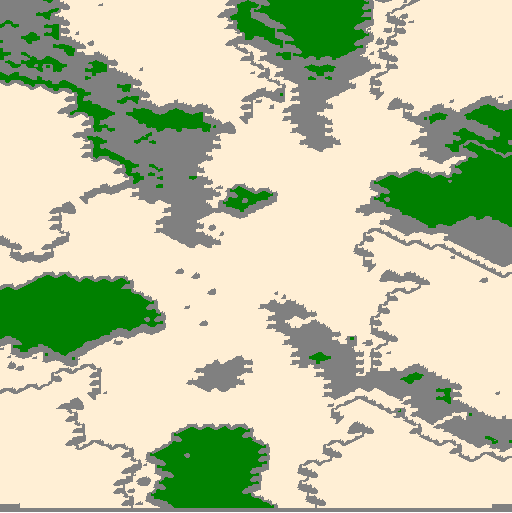
\includegraphics[width=10cm]{./img/Aftershock.png}
\caption{Graf \uv{Aftershock}}
\label{fig:aftershock_map}
\end{figure}
\begin{figure}[h]
\centering
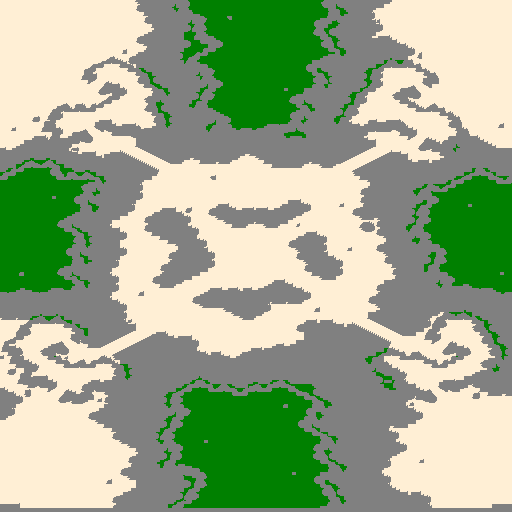
\includegraphics[width=10cm]{./img/Brushfire.png}
\caption{Graf \uv{Brushfire}}
\label{fig:brushfire_map}
\end{figure}
\subsection{Testovacie kritériá}
Algoritmy testujeme podľa nasledovných kritérií:

\begin{itemize}
\item Počet prehľadaných vrcholov.
\item Rýchlosť nájdenia cesty.
\item Optimalita cesty. 
\end{itemize}


\subsection{Testované algoritmy}
Testovať budeme nasledujúce algoritmy:
\begin{itemize}
\item Dijkstrov algoritmus nad binárnou haldou (označíme DH).
\item Dijkstrov algoritmus nad priehradkovou haldou (označime DBQ).
\item A* používajúci 6 landmarkov (označíme A*).
\item A* používajúci 6 landmarkov a taktiež obdĺžnikovú dekompozíciu, popísanú v kapitole 3 (označíme A*+).
\item Anderson -- s prehľadom najrýchlejší algoritmus, ktorý vyhral súťaž (označíme And).
\end{itemize}


\subsection{Kompilácia}
Kód bude kompilovaný kompilátorom g++. Bude porovnaná
rýchlosť behu programu pri kompilácii s direktivou \emph{g++ -O3}, čo zaručuje maximálnu rýchlosť a efektivitu behu programu.

\subsection{Typy máp a ciest}
Algoritmy budú testovane na troch mapách. 
Ich grafická reprezentácia je vytvorená v programe T-maps.
Popis programu sa nachádza v prílohách ~\ref{userdoc}~\ref{programdoc}.


V tabuľke \ref{fig:verticesscanned_result} ... Pozor, algoritmus And tu nienie TODO?? tri algoriymy rovnaky pocet

\section{Výsledky}
\begin{figure}[H]
	\centering
	\begin{tabular}{|l | r|r|r|r|}
	\hline
	 & AS & AL & BS & BL \\
	\hline
	DH, DBQ & 20888032 & 26585115 & 14967159 & 15403707 \\
	A*+ & 7694 & 115234& 7780 & 115234 \\
	\hline
	\end{tabular}
	\caption{Výsledky obsahujúce počet navštívených vrcholov}
	\label{fig:verticesscanned_result}
\end{figure}

\begin{figure}[H]
	\centering
	\begin{tabular}{|l | r|r|r|r|}
	\hline
	 & AS & AL & BS & BL \\
	\hline
	DH & 111010 & 548861 & 78330.7& 326556\\
	DBQ & 8710.17 & 548861 & 8731.65 & 152185 \\
	A* & 8743.7 & 144527& 8762.74 & 153288 \\
	A*+ & 8738.43& 144527 & 8758.98 & 153288 \\
	And & 22057.2 & 144854 & 22010 & 156927 \\
	\hline
	\end{tabular}
	\caption{Výsledky obsahujúce prejdeny vzialenosť}
	\label{fig:totalpath_result}
\end{figure}

\begin{figure}[H]
	\centering
	\begin{tabular}{|l | r|r|r|r|}
	\hline
	 & AS & AL & BS & BL \\
	\hline
	DH & 8.706919 & 8.609133 & 4.554813 & 3.803920 \\
	DBQ & 0.506893 & 11.505914 &  0.329444 & 4.315670\\
	A* & 0.263951 & 7.481771 & 0.283890 & 15.599357 \\
	A*+  & 0.182731 & 7.502437 &  0.197504 & 15.670339 \\
	And  &  0.000543 & 0.002659 & 0.000359 & 0.001747\\
	\hline
	\end{tabular}
	\caption{Výsledky časov v sekundách}
	\label{fig:totaltime_result}
\end{figure}
